
\documentclass[a4 paper,12pt]{article}
\usepackage[inner=2.0cm,outer=2.0cm,top=2.5cm,bottom=2.5cm]{geometry}
\usepackage{setspace}
\usepackage{appendix}
\usepackage[rgb]{xcolor}
\usepackage{tabu}
\usepackage{multirow}
\usepackage{longtable}
\usepackage{graphicx}
\usepackage{verbatim}
\usepackage{longtable}
\usepackage{subcaption}
\usepackage{fancyhdr}
\usepackage[colorlinks=true, urlcolor=blue, linkcolor=blue, citecolor=blue]{hyperref}
\usepackage{booktabs}
\usepackage{amsmath,amsfonts,amsthm,amssymb}
\usepackage{setspace}
\usepackage{fancyhdr}
\usepackage{lastpage}
\usepackage{tikz}
\usepackage{listings}
%\lstset{
	%	commentstyle=\color{red!50!green!50!blue!50},%代码块背景色为浅灰色
	%	rulesepcolor= \color{gray}, %代码块边框颜色
	%	breaklines=true,  %代码过长则换行
	%	numbers=left, %行号在左侧显示
	%	numberstyle= \small,%行号字体
	%	keywordstyle= \color{blue},%关键字颜色
	%	frame=shadowbox,%用方框框住代码块
	%	basicstyle=\ttfamily
	%}
\definecolor{dkgreen}{rgb}{0,0.6,0}
\definecolor{mauve}{rgb}{0.9,0.1,0.4}
\definecolor{ash}{rgb}{0.8,0.8,0.8}
\lstset{ 
	language=Octave,                % the language of the code
	basicstyle=\ttfamily,           % the size of the fonts that are used for the code
	numbers=left,                   % where to put the line-numbers
	numberstyle=\small\color{gray},  % the style that is used for the line-numbers
	stepnumber=2,                   % the step between two line-numbers. If it's 1, each line
	% will be numbered
	numbersep=5pt,                  % how far the line-numbers are from the code
	backgroundcolor=\color{ash},      % choose the background color. You must add \usepackage{color}
	rulesepcolor= \color{gray}, %代码块边框颜色
	showspaces=false,               % show spaces adding particular underscores
	showstringspaces=false,         % underline spaces within strings
	showtabs=false,                 % show tabs within strings adding particular underscores
	frame=single,                   % adds a frame around the code
	rulecolor=\color{black},        % if not set, the frame-color may be changed on line-breaks within not-black text (e.g. commens (green here))
	tabsize=2,                      % sets default tabsize to 2 spaces
	captionpos=b,                   % sets the caption-position to bottom
	breaklines=true,                % sets automatic line breaking
	breakatwhitespace=false,        % sets if automatic breaks should only happen at whitespace
	title=\lstname,                   % show the filename of files included with \lstinputlisting;
	% also try caption instead of title
	frame=shadowbox,%用方框框住代码块
	keywordstyle=\color{blue},          % keyword style
	commentstyle=\color{dkgreen},       % comment style
	stringstyle=\color{mauve},         % string literal style
	escapeinside={\%*}{*)},            % if you want to add LaTeX within your code
	morekeywords={*,...}               % if you want to add more keywords to the set
}
\usetikzlibrary{positioning, arrows.meta}
\usepackage{extramarks}
\usepackage{ctex,amsmath,amsfonts,amssymb,bm,hyperref,graphicx}
\usepackage{chngpage}
\usepackage{soul,color}
\usepackage{graphicx,float,wrapfig}
\newcommand{\homework}[3]{
	\pagestyle{myheadings}
	\thispagestyle{plain}
	\newpage
	\setcounter{page}{1}
	\noindent
	\begin{center}
		\framebox{
			\vbox{\vspace{2mm}
				\hbox to 6.28in { {\bf 现代电子电路基础及实验报告 \hfill} {\hfill {\rm #2} {\rm #3}} }
				\vspace{4mm}
				\hbox to 6.28in { {\Large \hfill #1  \hfill} }
				\vspace{3mm}}
		}
	\end{center}
	\vspace*{4mm}
}
\newcommand\numberthis{\addtocounter{equation}{1}\tag{\theequation}}

\begin{document}
	\homework{集成运算放大器的应用(二)}{1900011413}{吴熙楠}
	
	\section{实验目的}
	(1)通过实验进一步了解运算放大器的基本特性;
	\par (2) 进一步学习并掌握运算放大器的应用;
    \par (3)进一步练习插接,掌握调试技术和测量频率的方法;
    \par (4)研究振荡器的起振条件和振荡频率;
    \par (5)观察负反馈对振荡波形的影响。
	\section{实验器材}
	直流稳压电源、示波器、信号发生器、万用表、面包板 、运算放大器,电阻,电容,二极管,三极管。
	\section{实验原理}
    \noindent
\textbf{3.1\quad RC晶体管振荡器}
\par 如图所示是用晶体管组成的桥式正弦波振荡器电路,由两部分组成,虚线左边是振荡器反馈网络,右边则是放大器部分。
		\begin{figure}[H]
		\centering
		\hspace{2em}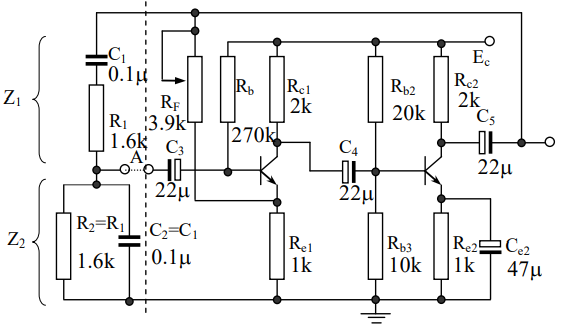
\includegraphics[width=.5\linewidth]{pic/1.png}
		\caption{\small{RC桥式振荡器电路图}
		}
	\end{figure}
    \par 对于这样的电路起振条件为:$|\dot{A}\dot{F}|\geq1,\phi_{A}+\phi_{F}=2n\pi \quad(n=0,1,2,3,\cdots)$
    \par 这个条件将使得振荡器振幅越来越大,为了达到稳幅振荡状态,需要在放大器或反馈网络中引入由非线性元件组成的稳幅环节。
    \par 由于我们可以计算出在$\omega=\dfrac{1}{RC}$时,|$\dot{F}$|=$\dfrac{1}{3}$,$\phi_{F}=0$
    \par 由于反馈网络特性确定,所以需要放大器满足$\phi_{A}=2n\pi,|A|\geq3$,并要求有很大的输入阻抗和很小的输出阻抗,以免影响反馈网络,所以我们通常在放大器中引入较深的负反馈来达到要求。\\
    \textbf{3.2\quad 利用运算放大器做积分运算}
    \par 积分电路具有反相输入结构,由于运放工作在线性区,可以计算得$u_{o}=-\dfrac{1}{R_{1}C}\int u_{i} dt$,积分电路图如下所示:
 		\begin{figure}[H]
 		\centering
 		\hspace{2em}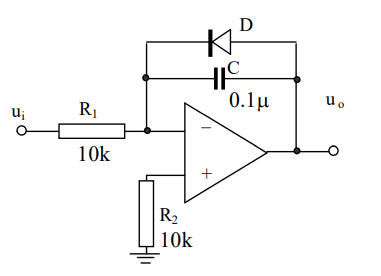
\includegraphics[width=.5\linewidth]{pic/2.png}
 		\caption{\small{积分电路图}
 		}
 	\end{figure}   
    \textbf{3.3\quad 利用运算放大器做微分运算}
        \par 微分是积分的逆运算,所以理论上只要将积分电路的电容和电阻对换位置,就成了微分电路,可以计算得$u_{o}=-RC\dfrac{du_{i}}{dt}$,微分电路图如下所示:
     		\begin{figure}[H]
     		\centering
     		\hspace{2em}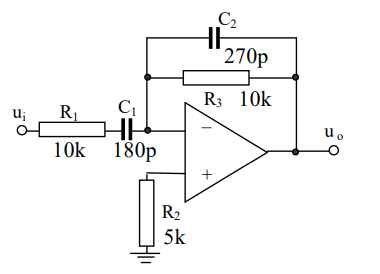
\includegraphics[width=.5\linewidth]{pic/3.png}
     		\caption{\small{微分电路图}
     		}
     	\end{figure}
	\section{实验内容}
    \noindent
\textbf{4.1\quad RC晶体管振荡器}
\par 根据实验数据可得:$R_{F}=1.9275k\Omega,u_{o}=6.4V,u_{i}=2.0V,f=1.092kHz$
\par 所以我们可得:$A_{F}=\dfrac{u_{o}}{u_{i}}=3.2>3$,我们与理论值比较可得:$A_{F}=1+\dfrac{R_{F}}{R_{P}}\approx 2.93$,可见我们测的实际值与理论值相差不大
\par 根据理论计算$f=\dfrac{1}{2\pi RC}\approx1.061kHz,$而我们实际测得$f=1.092kHz$,可见振荡频率实际值与理论值也十分吻合
\par 下图为RC振荡器自激振荡后波形图:
		\begin{figure}[H]
		\centering
		\hspace{2em}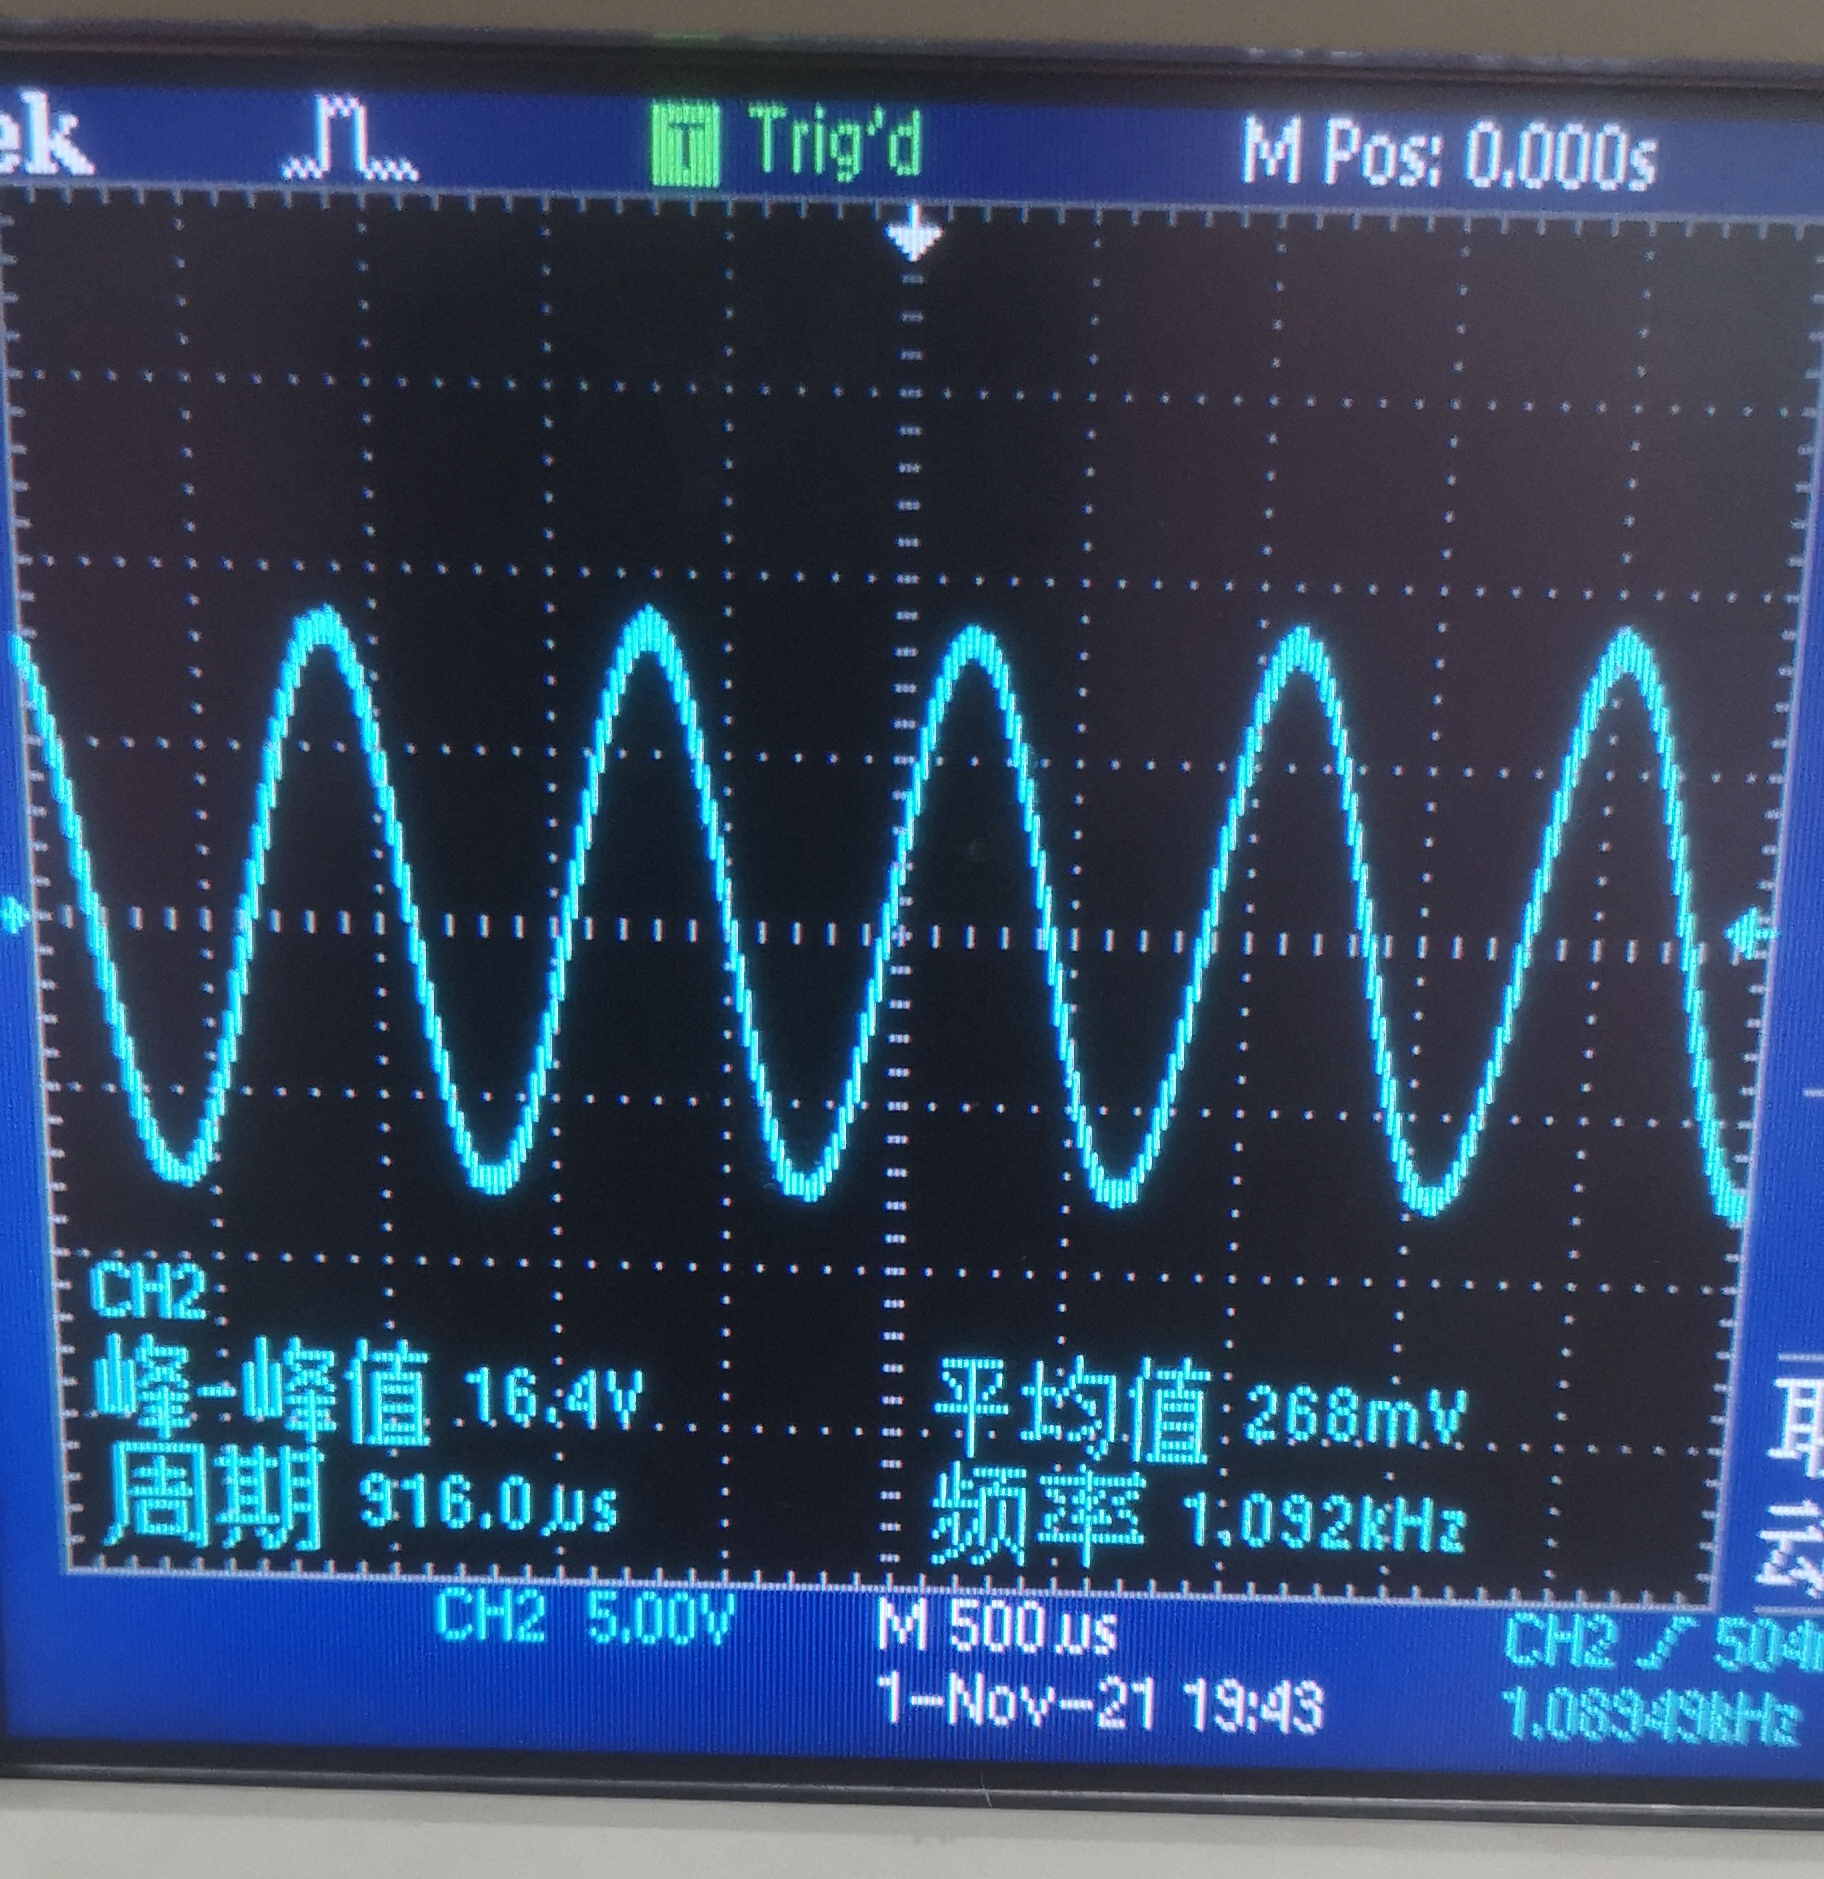
\includegraphics[width=.4\linewidth]{pic/1.jpg}
		\caption{\small{RC振荡器自激振荡波形图}
		}
	\end{figure}
\noindent    
\textbf{4.2\quad 利用运算放大器做积分运算}
\par 输入方波后积分计算波形图如图所示:
		\begin{figure}[H]
		\centering
		\hspace{2em}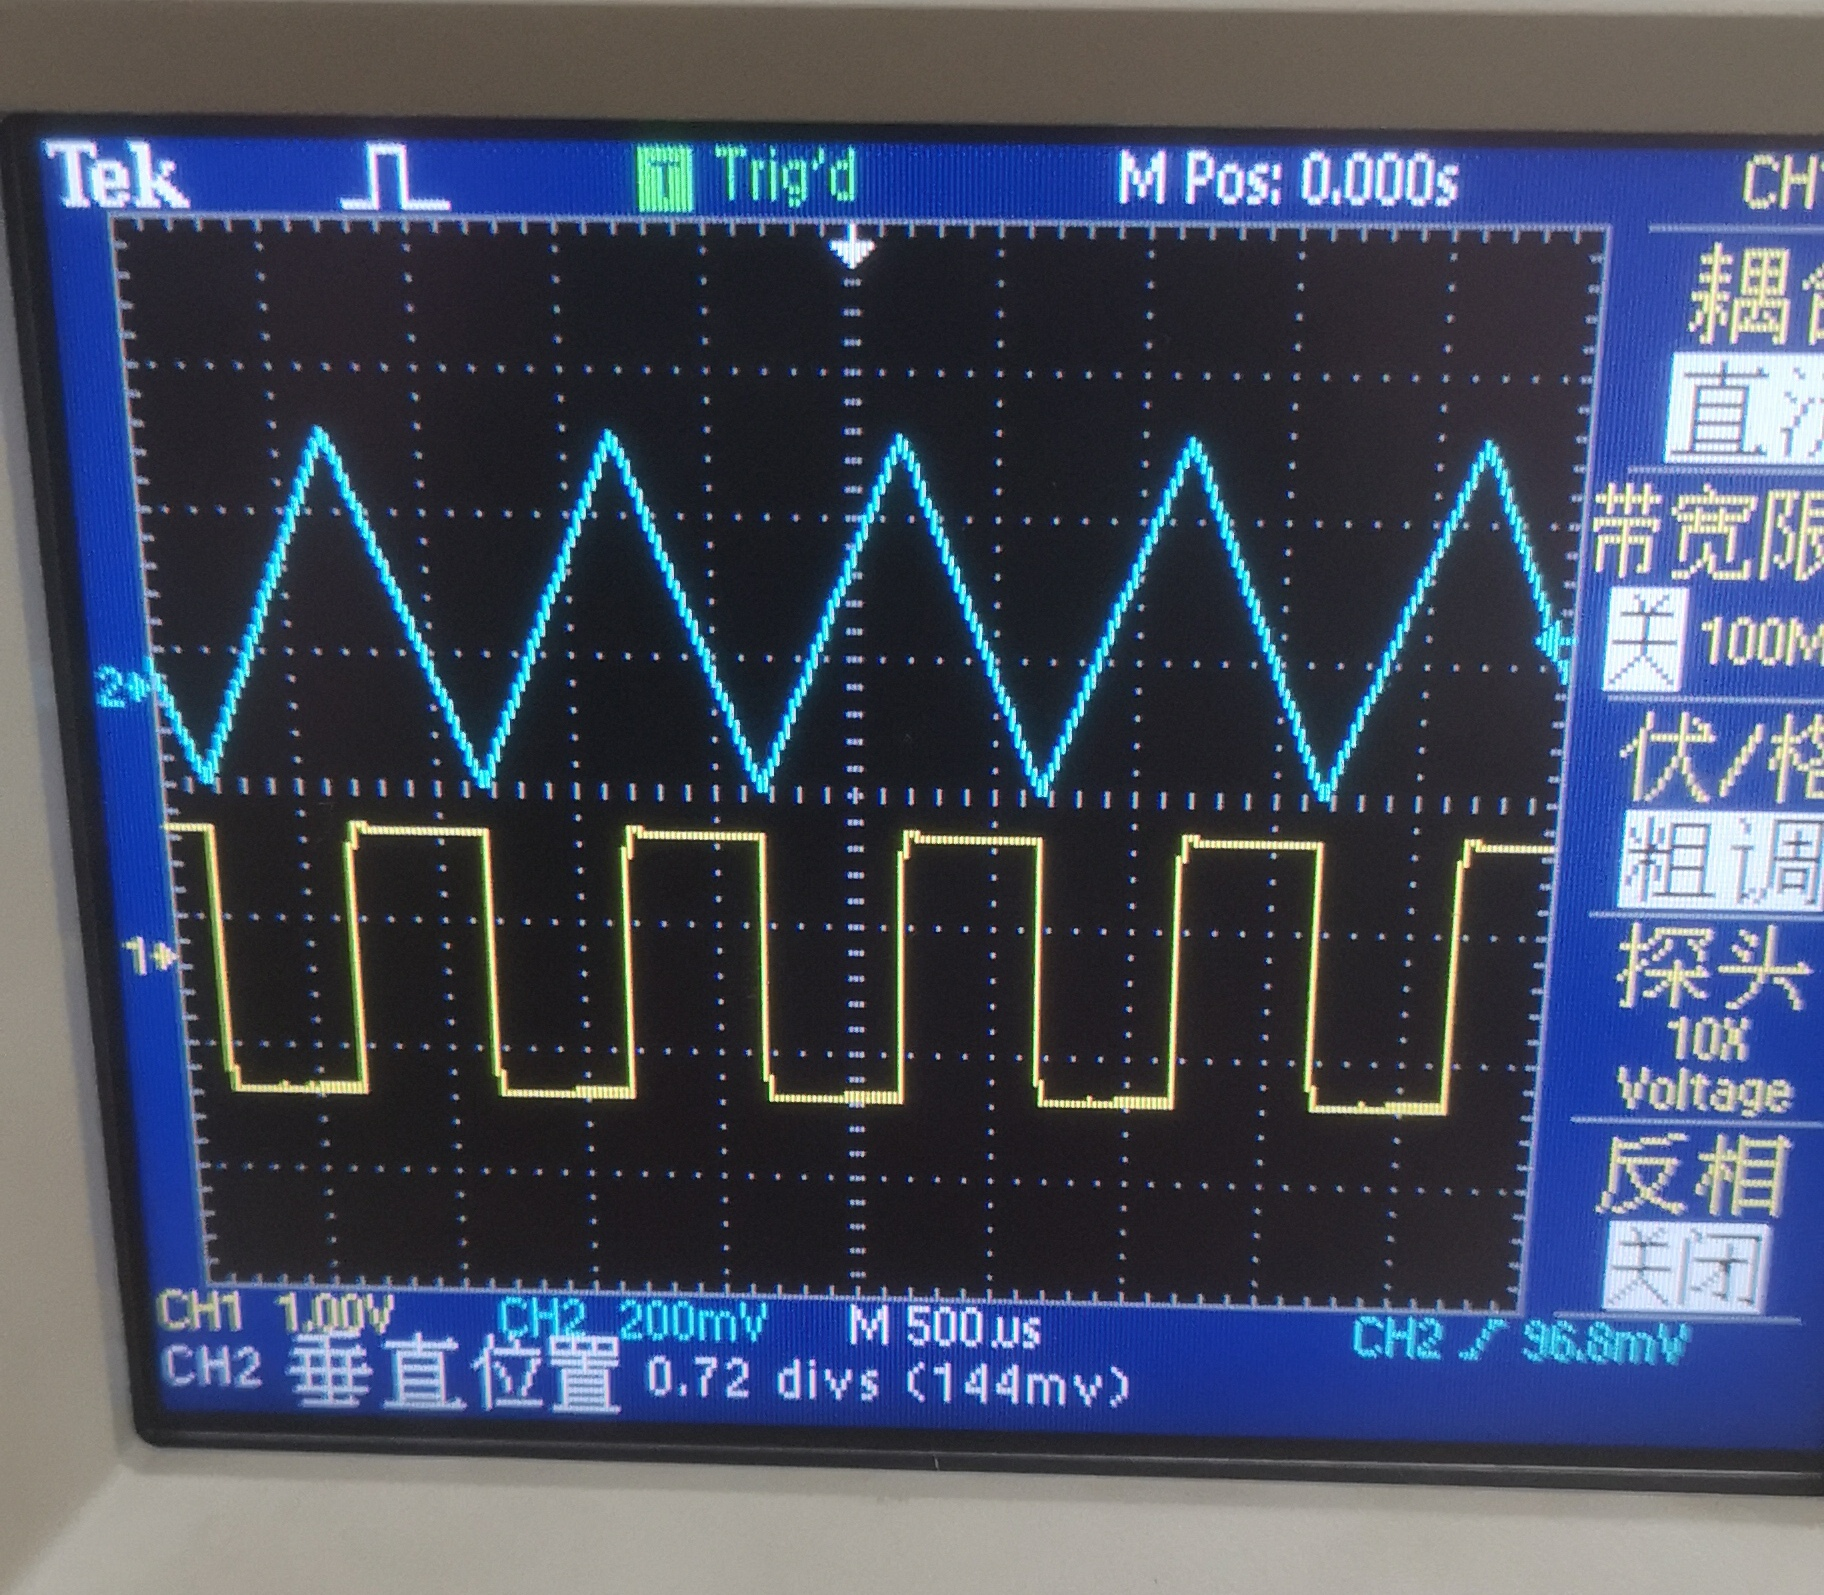
\includegraphics[width=.4\linewidth]{pic/2.jpg}
		\caption{\small{方波积分计算波形图}
		}
	\end{figure}
    \par 由图中可见输入方波相位与输出的三角波的相位相反(即方波处于高电平时三角波为上升期,方波处于低电平时三角波为下降期)
    \par 我们可以得到实验数据为:$T=2\times 416\mu s=832\mu s,u_{p-p}=508mV,$我们输入的$u_{i}=0.5\times 2.0V=1.0V$
    \par 因此我们实测的输出三角波的斜率为:$k=\dfrac{508mV}{416\mu s}=1.221\times 10^{3}V/s$,而理论计算应该为:$k=\dfrac{u_{i}}{RC}=\dfrac{1.0V}{10^{-3}s}=1.0\times 10^{3}V/s$,可见实测值与理论值相差也不大
    
\noindent
\textbf{4.3\quad 利用运算放大器做微分运算}
\par 输入方波后微分计算波形图如图所示:
		\begin{figure}[H]
		\centering
		\hspace{2em}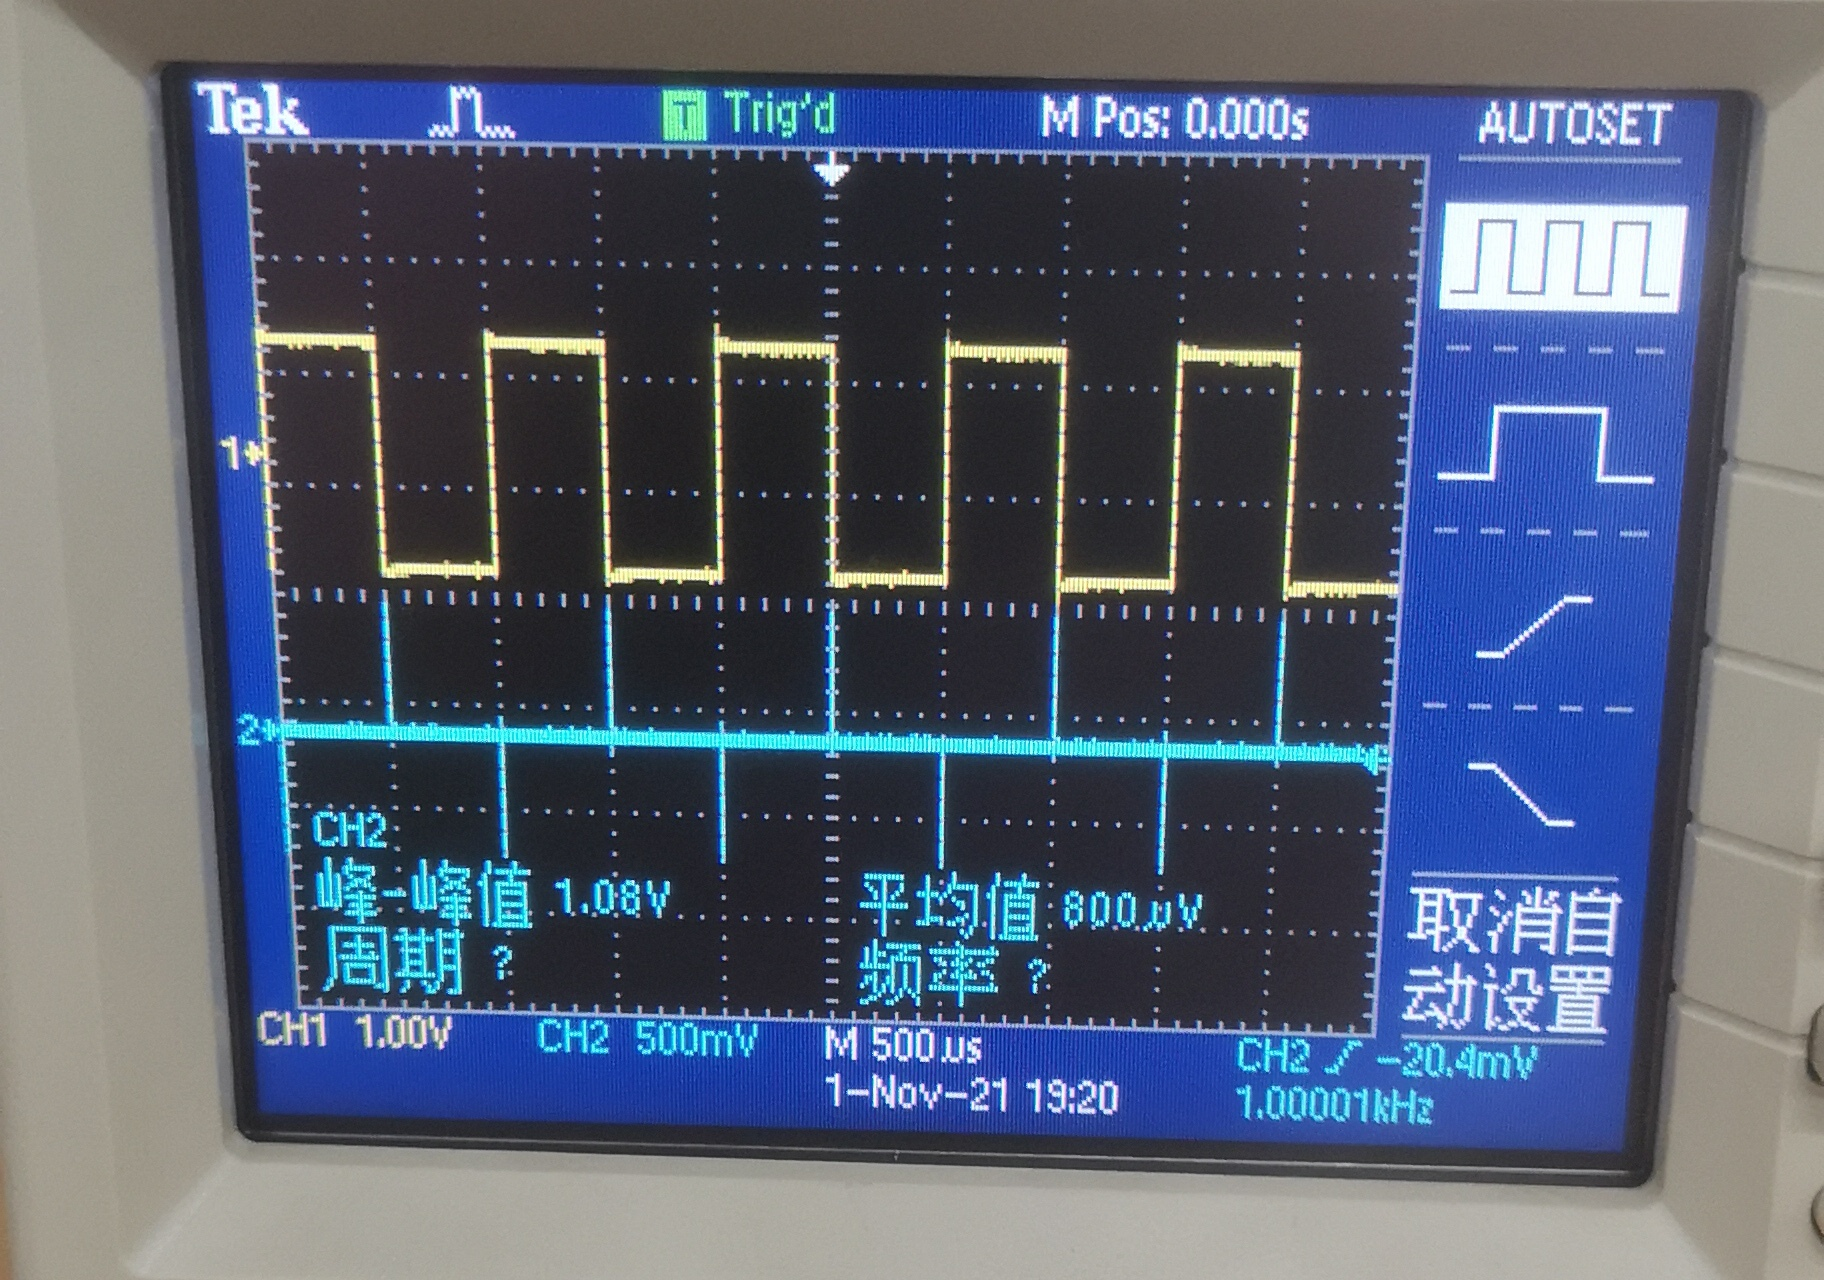
\includegraphics[width=.4\linewidth]{pic/3.jpg}
		\caption{\small{方波微分计算波形图}
		}
	\end{figure}
    \par 可见在每个方波的高电平和低电平时,输出均为$0V$,而当方波处于上升沿或者下降沿时,输出会出现一个峰值,且相位与输入方波相反,即上升沿处的输出为负值,下降沿处的输出为正值。
	\section{思考题}
	\noindent
	\textbf{1.运放哪些应用是分别利用了运放的线性特性、非线性特性?
}
	\par 答:线性特性应用:理想运算放大器的虚短路与虚断路特性,反相比例放大器,同相比例放大器,反相与同相加减法电路,有源低通滤波器,有源高通滤波器等;非线性特性应用:方波发生器,滞回比较器,双向限幅比较器等。\\
    \textbf{2.在本电路中采用什么措施可以使电路自动起振并能使振幅稳定?}
    \par 答:在本电路中使得$|\dot{A}\dot{F}|>1,|\dot{F}|=\dfrac{1}{3},|\dot{A}|>3$,以及$\phi_{A}=2n\pi \quad(n=0,1,2,3,\cdots)$,这时的条件可以使得电路自动起振;为了达到稳幅振荡状态,需要在放大器或反馈网络中引入由非线性元件组成的稳幅环节,以及增加负反馈调节网络来稳定振幅。
\end{document} 
